This appendix records the literature search used in Chapter~2. It is not a claim that every
bibliography entry in the dissertation was retrieved by that screen. A systematic open-literature
pass identified 53 candidate records, excluded 7 at full text, and retained 46 in the synthesis
matrix. Chapter~2 also cites already-admitted UK-register, governance and vendor sources that sat
outside that screen. The dissertation's admitted citation pool is therefore larger than the matrix
$N$. The full matrix is stored as \texttt{sources/literature\_synthesis\_matrix.tsv}.

\section*{PRISMA-style flow}

\begin{table}[htbp]
  \centering
  \small
  \begin{tabularx}{\textwidth}{@{}P{0.38\textwidth}P{0.12\textwidth}Y@{}}
    \toprule
    \textbf{Stage} & \textbf{Count} & \textbf{Notes} \\
    \midrule
    Candidate records screened & 53 & Open-literature pass across five theme searches \\
    Duplicates removed & 0 & Theme-partitioned searches; no exact duplicates \\
    Full-text screened & 53 & English; agent and language-model work from 2022 \\
    Excluded at full text & 7 & Reasons in the table below \\
    Included in the synthesis matrix & 46 & Readable subset below; full TSV in the repository \\
    \bottomrule
  \end{tabularx}
  \caption{PRISMA-style identification and screening counts}
  \label{tab:lit-prisma-flow}
\end{table}

Grey literature was admitted only for governance or market context and is labelled as such in the
matrix. Google Scholar was used only to chase citations of already included papers. The Boolean
strings are stored in \texttt{sources/literature\_search\_log.tsv}.

\section*{Sources screened out at full text}

\begin{table}[htbp]
  \centering
  \small
  \begin{tabularx}{\textwidth}{@{}P{0.46\textwidth}Y@{}}
    \toprule
    \textbf{Source} & \textbf{Reason for exclusion} \\
    \midrule
    Maier et al.\ (2015), SROI merits and limitations & Redundant with an included systematic SROI review \\
    Tiron-Tudor et al.\ (2024), RPA in accounting & Adjacent corporate RPA domain, not venture reporting \\
    Madaan et al.\ (2023), Self-Refine & Overlaps Reflexion on the generator--critic pattern \\
    Dhuliawala et al.\ (2023), Chain-of-Verification & Attribution already saturated; no external grounding \\
    Bohnet et al.\ (2022), Attributed QA & Short-answer attribution; less central than ALCE/RARR \\
    Stureborg et al.\ (2024), inconsistent evaluators & Judge-bias already covered by included sources \\
    FCA (2024) AI research note & Companion overlap with already admitted FCA guidance \\
    \bottomrule
  \end{tabularx}
  \caption{Full-text exclusions from the systematic screen}
  \label{tab:lit-screened-out}
\end{table}

These seven items are the screen exclusions. They are not the same list as the separate UK
data-access gate used for implementation sources, recorded under
\texttt{research/literature/} as \texttt{REJECTED\_CANDIDATES.md}.

\section*{Imported sources used in Chapter~2}

\begin{table}[htbp]
  \centering
  \scriptsize
  \setlength{\tabcolsep}{3pt}
  \begin{tabularx}{\textwidth}{@{}P{0.28\textwidth}P{0.22\textwidth}Y@{}}
    \toprule
    \textbf{Source} & \textbf{Home in Chapter~2} & \textbf{Job in the argument} \\
    \midrule
    Panickssery, Bowman and Feng (2024) & §2.4 & Verifier must not rewrite the claim; self-preference is a demonstrated failure mode \\
    Yue et al.\ (2023) & §2.4 & Contradiction detection is weak, so conflict is retained for a named person \\
    Min et al.\ (2023) & §2.4 & Verification is claim-level, not report-level \\
    Fu et al.\ (2026), preprint & §2.6 & Matched inputs are the only credible test; warrant for C1/C2 \\
    Du, Shinn, Hong and Qian & §2.6 & Position~A: named roles can help when a checkable signal exists \\
    Kamoi et al.\ (2024); Thorat, Laban and Wu (2024) & §3.4, §5.4 & Error-detection and error-injection warrant for D0; not comparable with C2 \\
    \bottomrule
  \end{tabularx}
  \caption{Sources imported into the rebuilt Chapter~2 argument}
  \label{tab:lit-imported-sources}
\end{table}

The matrix also includes sources that this dissertation does not cite, including promised manual
baselines, expert ratings and usability studies that were never run. Those items remain in the
repository file. They are not used as evidence in the body.

\clearpage
\begin{figure}[htbp]
  \centering
  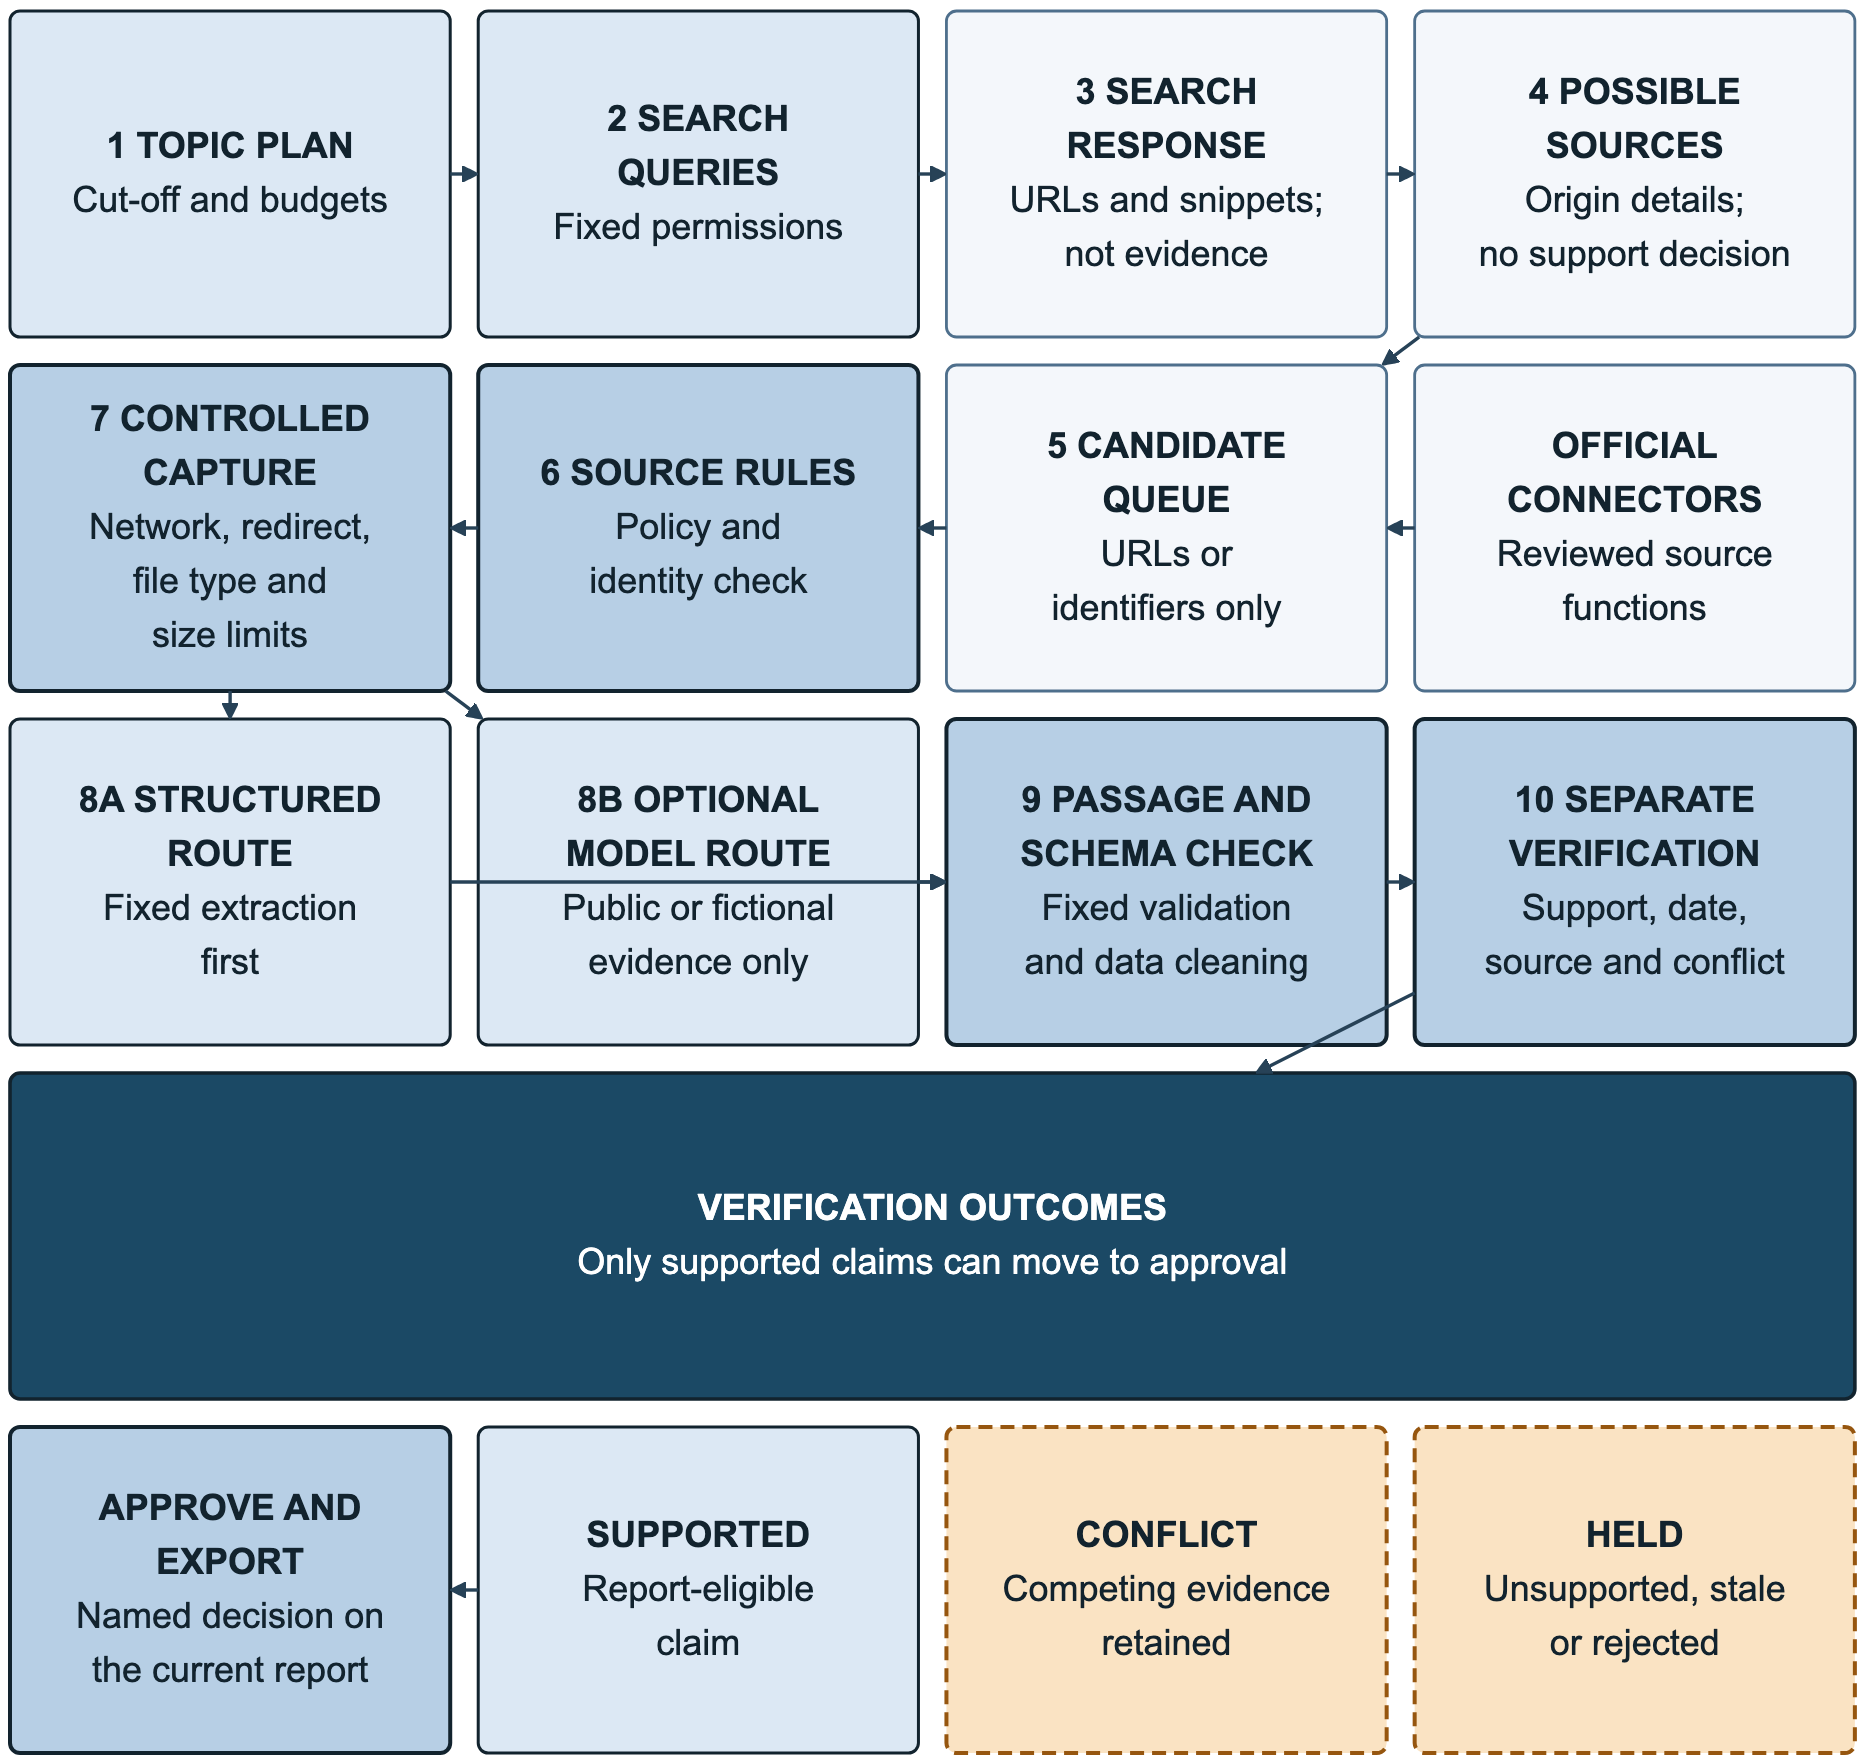
\includegraphics[width=\textwidth,height=0.78\textheight,keepaspectratio]{exhibits/lit_f2_discovery_is_not_evidence.png}
  \caption{Why finding a source is not the same as having evidence. Developed by the author from the
  cited literature and the project's fixed rules.}
  \label{fig:lit-discovery-evidence-boundary}
\end{figure}
\clearpage

